\subsubsection{Learning outcomes}
For the writing skill module workshop I propose an additional learning outcome in each semester, namely communication in a written format.

\begin{figure*}[h!]
\begin{tabular}{|p{\textwidth}|}
 \hline
    \textbf{Learning outcome Semester 3: Basic communication writing skills}\\
    Communicate in a specific written task in the most appropriate manner.\\
 \hline
    \textit{Explanation}\\
    You use basic stylistic considerations and you are aware of your stylistic choices.
    \\ 
    You communicate information smoothly, using logical connections between ideas.\\
 \hline
\end{tabular}

\begin{tabular}{|p{\textwidth}|}
 \hline
    \textbf{Learning outcome Semester 6: Advanced communication writing skills}\\
    Communicate in a specific written task in the most appropriate manner.\\
 \hline
    \textit{Explanation}\\
    You use an appropriate/predictable format/pattern for a particular type of text (e.g. summary, introduction, data commentary).
    \\ 
 \hline
\end{tabular}
  \caption{Learning outcome for Semester 3 and Semester 6}
\end{figure*}

\begin{figure}[h!]
    \centering
   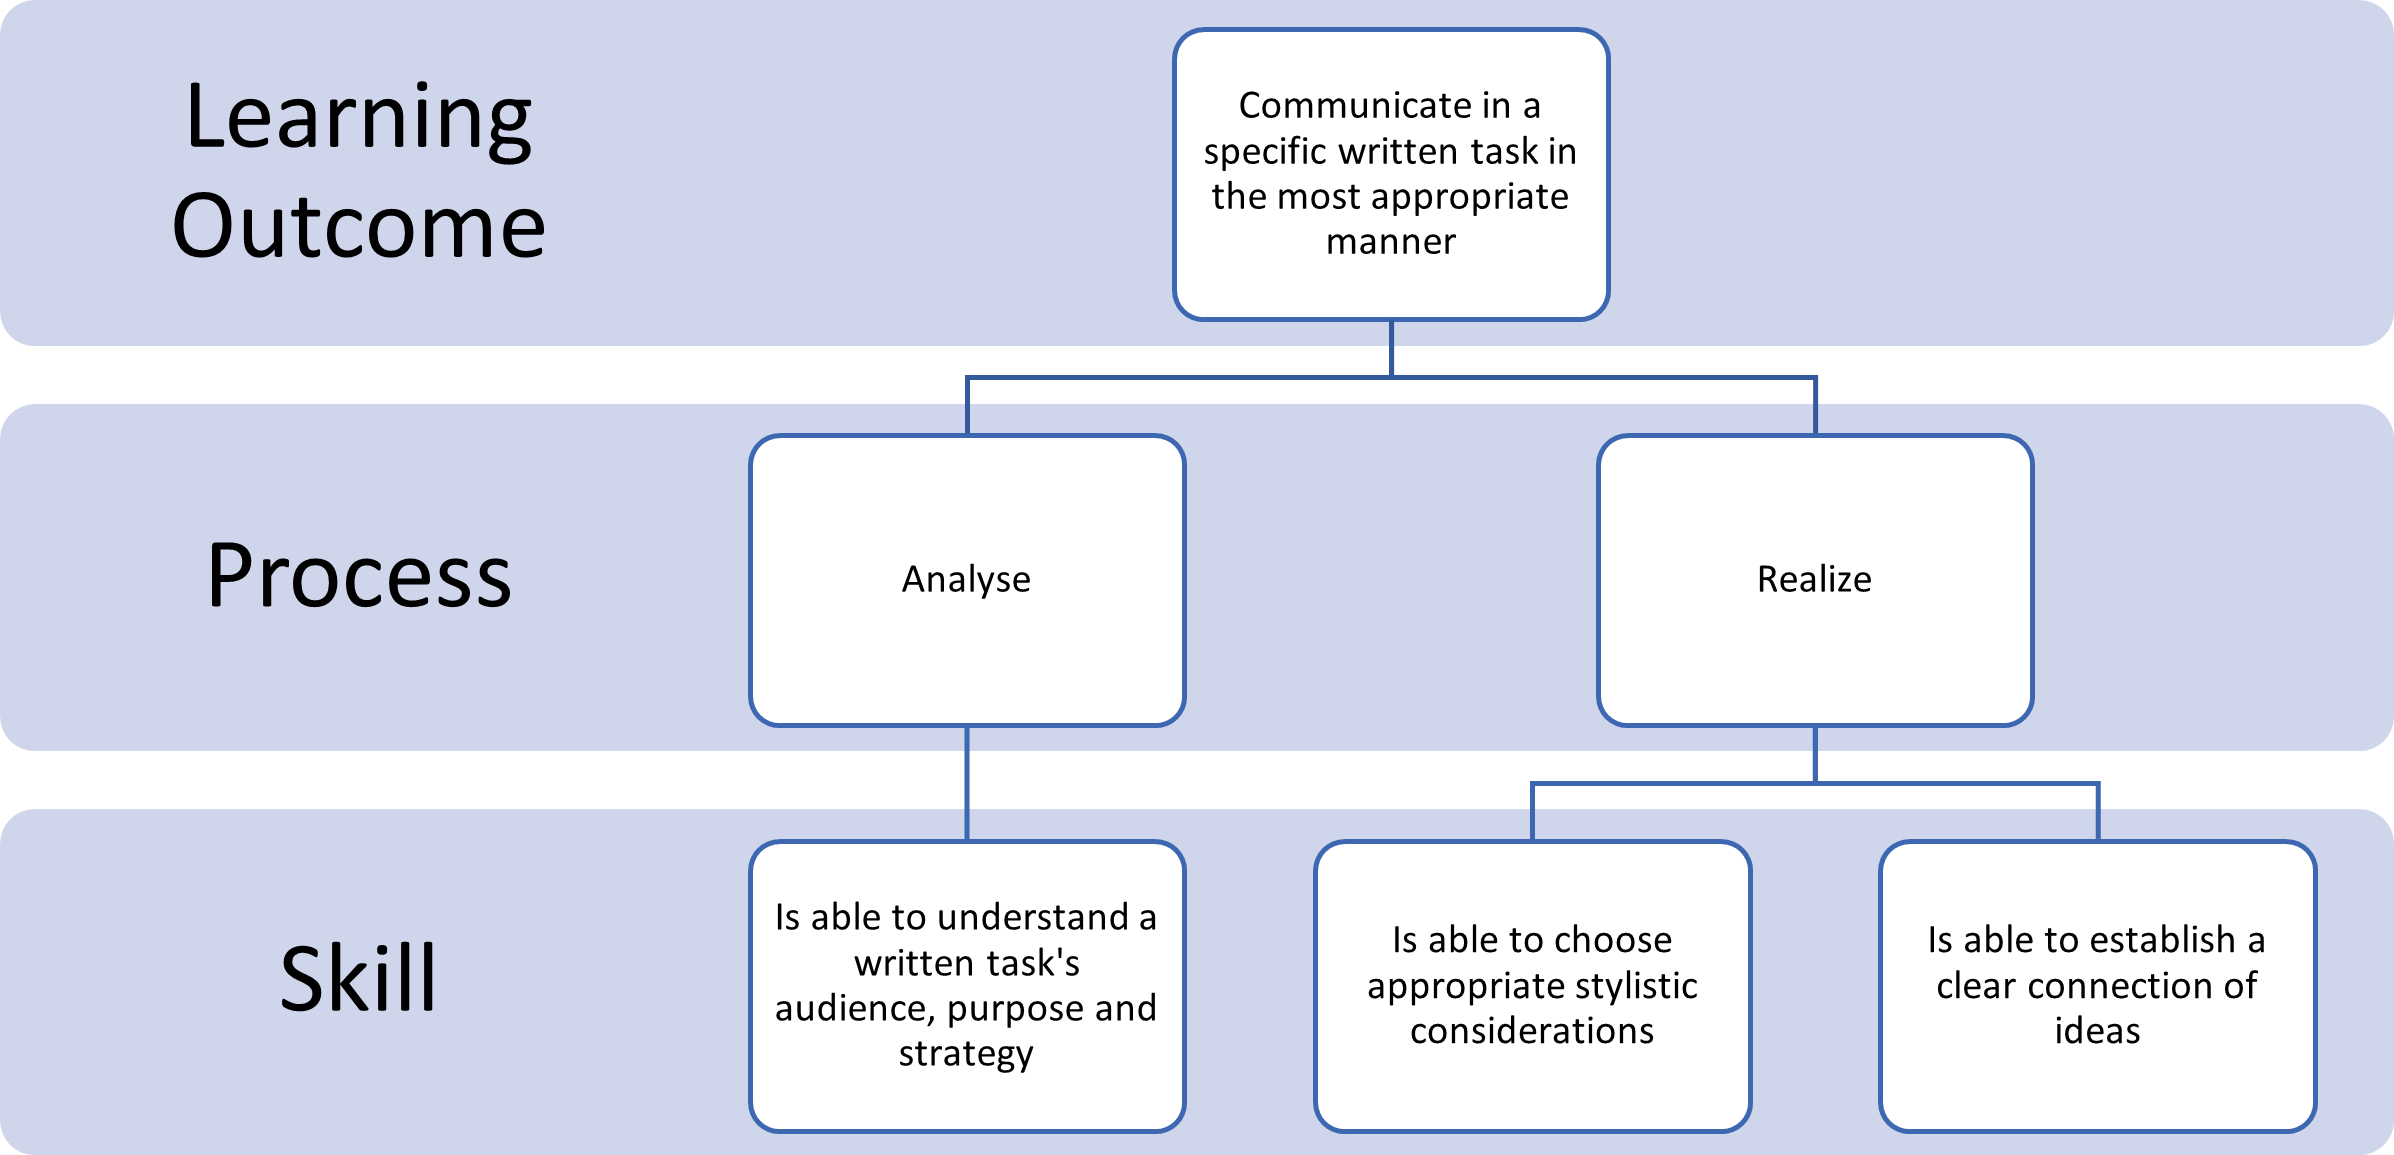
\includegraphics[width=\textwidth]{appendices/learning_outcomes/LO_S3.png}
    \caption{Skill tree for Semester 3 learning outcome: Basic communication writing skills}
    \label{fig:LO_S3}
\end{figure}

\begin{figure}[h!]
    \centering
   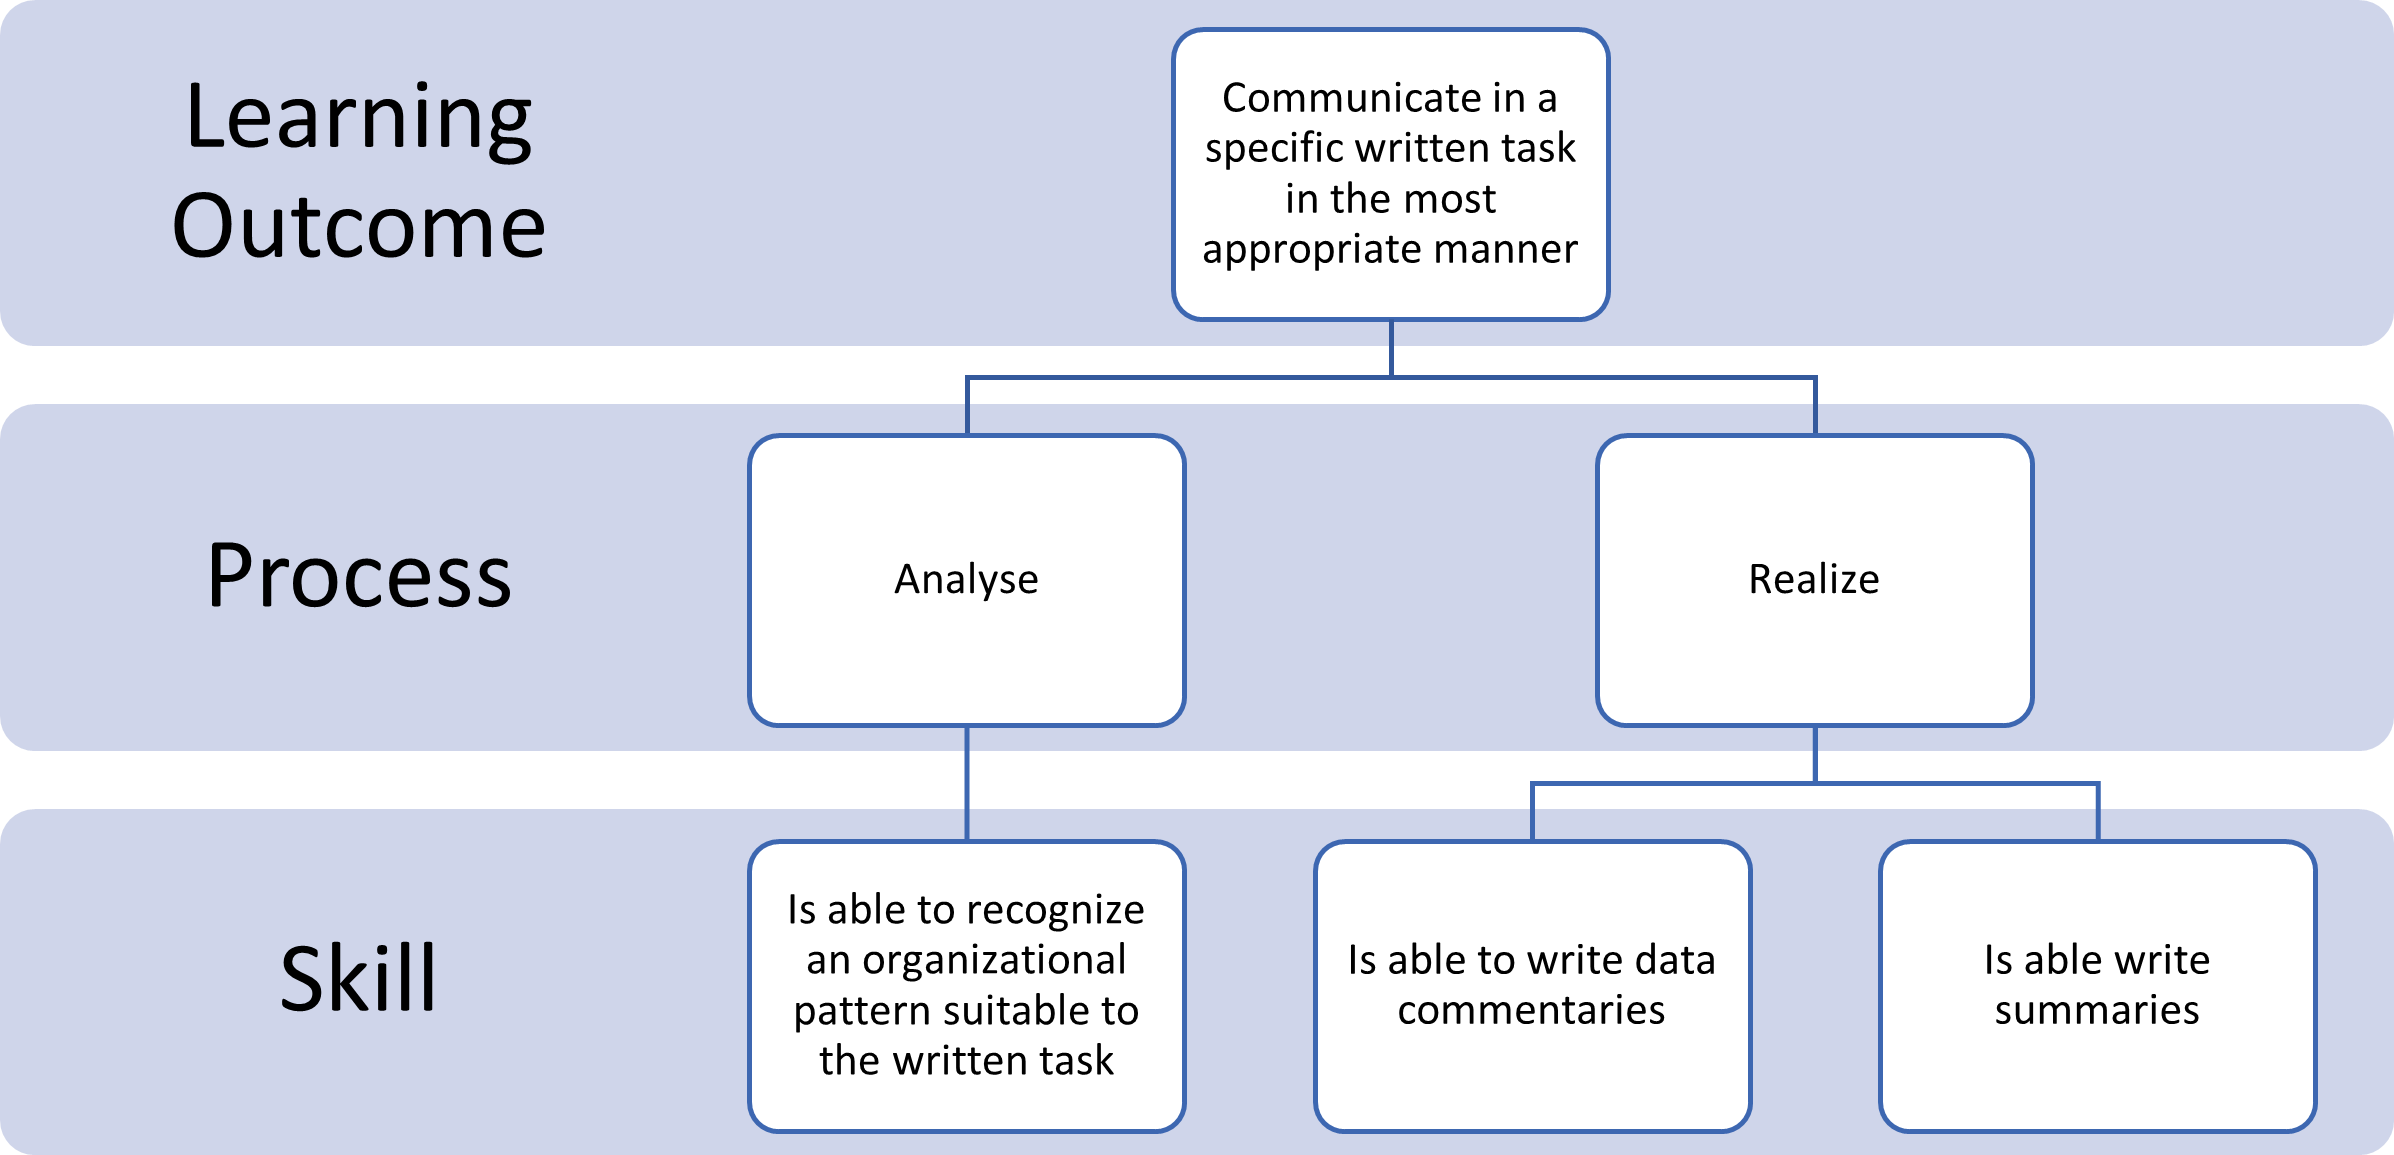
\includegraphics[width=\textwidth]{appendices/learning_outcomes/LO_S6.png}
    \caption{Skill tree for Semester 6 learning outcome: Advanced communication writing skills}
    \label{fig:LO_S6}
\end{figure}

\subsubsection{Learning activities}

The employed teaching method closely follows the \acrshort{4cid} model~\cite{FHICTTeachingMethods}. This model describes four basic components fitted to the course as follows:
\begin{itemize}
    \item learning tasks (weekly theory and practical lessons)
    \item supportive information (course notes and worked out examples, explanation of basics)
    \item practice tasks (individual tasks that aid to better understanding of topic)
    \item procedural information (feedback and feed forward through weekly individual short progress meetings)
\end{itemize}
